\chapter{Aufgaben}

Die folgenden Aufgaben bauen aufeinander auf. Zuerst geht es darum, den erklärten Code wirklich verstanden zu haben, danach folgt eine Rechenaufgabe zum DDS-Prinzip, und zum Schluss zwei offene, kreative Aufgaben, bei denen du selbst etwas entwirfst. Für die Rechenaufgabe findest du am Ende des Kapitels eine Lösung, für die kreativen Aufgaben gibt es bewusst keine Musterlösung.

\section{Fehlende Codeteile rekonstruieren}
\label{sec:fehlende-codeteile}

In eurem Projektordner sind an einigen Stellen Codezeilen nicht mehr vorhanden, offenbar hat sich ein hungriger Wurm durch die Dateien gefressen. Die betroffenen Stellen sind mit \texttt{-- TODO} markiert. Arbeite die Module in dieser Reihenfolge durch, sie bauen von einfach zu anspruchsvoll aufeinander auf. Nach jedem Schritt kompilieren und die betroffene Wellenform am Oszilloskop prüfen, erst dann weiter zum nächsten Modul.

\subsection*{1. frequenzteiler.vhd}

Der Grundbaustein für alles Weitere, \texttt{tick\_out} muss alle \texttt{divisor\_in} Systemtakte für genau einen Takt auf \texttt{'1'} gehen. Dazu zählt \texttt{counter} bei jedem Takt hoch, bei Erreichen von \texttt{divisor\_in - 1} wird \texttt{counter} zurückgesetzt und \texttt{tick\_reg} für diesen einen Takt auf \texttt{'1'} gesetzt, sonst bleibt \texttt{tick\_reg} auf \texttt{'0'}. Ohne dieses Modul bekommt keiner der Generatoren sein \texttt{tick\_en}, es lohnt sich also, hier zuerst anzusetzen.

\subsection*{2. rect\_gen.vhd}

Der Rechteckgenerator ist der einfachste Fall, hier zählst du nur einen Zähler hoch und schaltest bei Erreichen einer Grenze um. Im \texttt{process} fehlt genau das, \texttt{counter} muss bei jedem \texttt{tick\_en}-Puls um 1 erhöht werden, und sobald er \texttt{ticks\_per\_phase} erreicht, muss er auf 0 zurückgesetzt und \texttt{state} umgeschaltet (invertiert) werden. Wie \texttt{state} danach den Ausgang steuert, steht schon fertig unten im Code, das musst du nicht anfassen.

\subsection*{3. dreieck\_gen.vhd}

Fast derselbe Zählermechanismus wie eben, nur zählt hier zusätzlich \texttt{current\_val} selbst hoch oder runter, gesteuert über \texttt{is\_rising}. Es fehlt Folgendes, wenn die Schrittdauer (\texttt{tick\_counter} gegen \texttt{ticks\_limit}) erreicht ist, muss \texttt{current\_val} je nach \texttt{is\_rising} um 1 erhöht oder verringert werden. Erreicht \texttt{current\_val} dabei \texttt{max\_val}, kippt \texttt{is\_rising} auf \texttt{'0'} (jetzt fallend), erreicht es \texttt{min\_val}, kippt es zurück auf \texttt{'1'} (jetzt steigend).

\subsection*{4. saegezahn\_gen.vhd}

Wieder derselbe Zählermechanismus, diesmal ohne Richtungswechsel, \texttt{current\_val} zählt nur hoch. Es fehlt, bei Erreichen der Schrittdauer entweder \texttt{current\_val} um 1 zu erhöhen, oder, falls \texttt{max\_val} bereits erreicht ist, hart zurück auf \texttt{min\_val} zu springen (kein Herunterzählen wie beim Dreieck).

\subsection*{5. Den SIN-Kern erzeugen}
\label{sec:sin-kern}

Für den nächsten Schritt, den Sinusgenerator, wird ein fertiger IP-Baustein für die Sinustabelle gebraucht. Die Datei \texttt{SIN.vhd} fehlt aktuell komplett und muss über IPexpress neu erzeugt werden, sonst lässt sich ab hier nichts mehr kompilieren (auch der Mystery-Modus aus Aufgabe~\ref{sec:mystery-melodie} braucht denselben Kern).

Öffne in Diamond den IP-Katalog und wähle unter \emph{Arithmetic\_Modules} das Modul \emph{Sin-Cos\_Table}. Trage im ersten Dialog als Dateiname \texttt{SIN} ein und wähle als Module Output \texttt{VHDL} (Abbildung~\ref{fig:sin1}).

\begin{figure}[H]
    \centering
    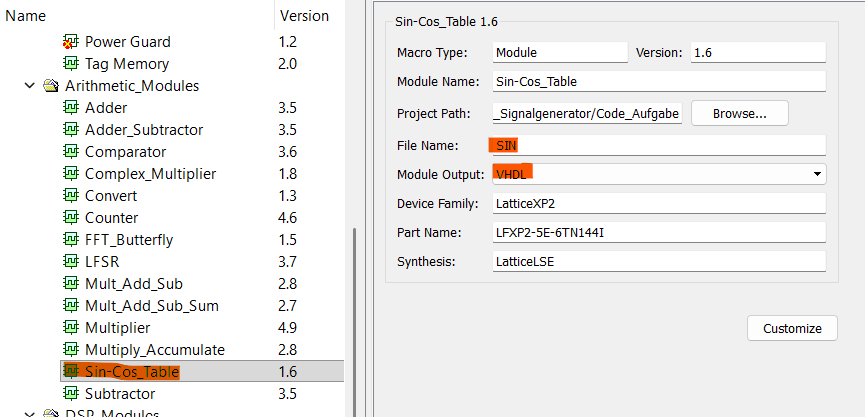
\includegraphics[width=14cm]{Bilder/SIN_1.png}
    \caption{IPexpress-Katalog, Modulauswahl Sin-Cos\_Table}
    \label{fig:sin1}
\end{figure}

Im Konfigurationsdialog müssen folgende Einstellungen gesetzt werden, damit der erzeugte Kern zum restlichen Code passt (Abbildung~\ref{fig:sin2}).

\begin{itemize}
    \item Input Theta Bit Width, \texttt{10}
    \item Output Mode, \texttt{Sin}
    \item \glqq Use Tables for Quarter-wave Only\grqq{} \textbf{nicht} angehakt
    \item Enable Input Registers und Enable Output Registers bleiben angehakt
\end{itemize}

\begin{figure}[H]
    \centering
    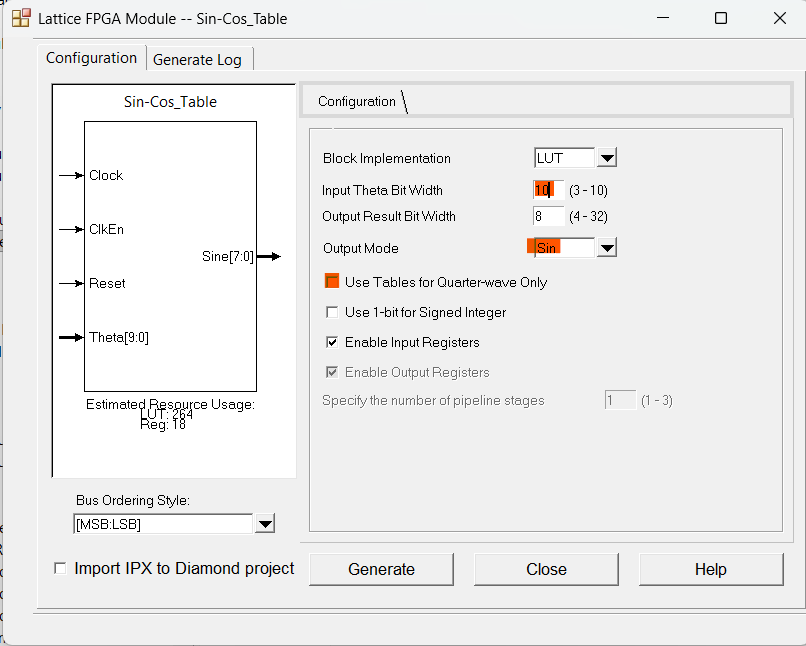
\includegraphics[width=10cm]{Bilder/SIN_2.png}
    \caption{IPexpress-Konfiguration, korrekte Einstellungen}
    \label{fig:sin2}
\end{figure}

Mit \emph{Generate} wird \texttt{SIN.vhd} neu erzeugt.

\subsection*{6. sinus\_gen.vhd}

Der eigentliche DDS-Kern aus Kapitel~\ref{ch:funktionsweise}, hier fehlt gleich zweimal etwas. Erstens muss \texttt{phase\_acc} bei jedem \texttt{tick\_en}-Puls um \texttt{phase\_inc} erhöht werden (auf die 10 Bit des Akkumulators resized). Zweitens, in der Skalierungspipeline nach dem SIN-Kern, muss \texttt{sine\_raw} vorzeichenrichtig auf 16 Bit erweitert, mit \texttt{amp\_in} multipliziert, um 8 Bit runterskaliert und danach um 128 verschoben werden, damit aus dem vorzeichenbehafteten Sinuswert (-128..127) ein für den DAC gültiger Wert (0..255) wird. Die genauen vier Schritte der Pipeline stehen als Kommentar im Code.

\subsection*{7. debounce.vhd}

Hier fehlt die eigentliche Entprellungslogik. \texttt{counter} muss hochzählen, solange sich \texttt{sync1} vom zuletzt übernommenen \texttt{stable\_val} unterscheidet. Erreicht \texttt{counter} dabei \texttt{DEBOUNCE\_CYCLES}, wird \texttt{sync1} als neuer \texttt{stable\_val} übernommen und \texttt{counter} zurückgesetzt. Stimmen \texttt{sync1} und \texttt{stable\_val} dagegen schon überein (kein Prellen mehr erkannt), wird \texttt{counter} ebenfalls zurückgesetzt.

\subsection*{8. steuerung.vhd}

Taster 5 (Wert erhöhen) ist bereits vollständig implementiert, schau ihn dir als Vorlage an. Es fehlt Taster 6 (Wert verringern), spiegelbildlich zu Taster 5, aber mit einer Besonderheit, \texttt{unsigned} kann nicht negativ werden. \texttt{p1\_reg} und \texttt{p2\_reg} müssen deshalb bei 1 stehen bleiben (nicht bei 0), \texttt{amp\_reg} bei 0.

\subsection*{9. toplevel.vhd}

Der letzte und wichtigste Schritt, der Multiplexer, der alle Generatoren zusammenführt. Erst wenn der steht, läuft das Gesamtsystem. Es fehlt eine \texttt{with sig\_mode select}-Zuweisung auf \texttt{final\_signal}, die je nach Modus die passende Wellenform durchreicht, \texttt{"001"} Sinus, \texttt{"010"} stumm (\texttt{x"00"}), \texttt{"011"} Dreieck, \texttt{"100"} Rechteck, \texttt{"101"} Sägezahn, \texttt{"110"} Mystery, alle anderen Werte ebenfalls stumm.

\section{Frequenzberechnung beim Sinusgenerator}
\label{sec:frequenzberechnung}

Der Sinusgenerator arbeitet nach dem DDS-Prinzip mit einem 10 Bit breiten Phasenakkumulator, ein voller Umlauf entspricht also 1024 Schritten. Der Phasenakkumulator wird bei jedem \texttt{tick\_en}-Puls um \texttt{P1} erhöht, und \texttt{tick\_en} selbst wird alle \texttt{P2} Systemtakte einmal aktiv, bei einem Systemtakt von 50\,MHz.

\begin{enumerate}
    \item Stelle eine Formel auf, die die Ausgabefrequenz $f_{\text{out}}$ in Abhängigkeit von \texttt{P1}, \texttt{P2} und dem Systemtakt beschreibt.
    \item Bestimme jeweils ein Wertepaar (\texttt{P1}, \texttt{P2}), mit dem der Sinusgenerator eine Ausgabefrequenz von etwa 100\,Hz beziehungsweise etwa 1\,kHz erzeugt. Das muss nicht exakt ausgerechnet sein, probier ruhig auch, bis es passt. Achte darauf, \texttt{P1} kleiner als 1024 zu wählen, größere Werte werden im Code auf 10 Bit gekürzt und ergeben dadurch eine andere Frequenz als erwartet.
    \item Stelle deine Werte ein und überprüfe direkt am Oszilloskop, ob die Frequenz stimmt.
\end{enumerate}

\section{Eigene Wellenform auf Modus X}

Modus 2 ist im Multiplexer des Toplevels aktuell auf stumm geschaltet und in der LED-Anzeige als \glqq X (deine Funktion)\grqq{} reserviert. Genau dafür ist er da.

Suche dir eine mathematische Funktion deiner Wahl aus, zum Beispiel eine Betragssinuskurve, eine Exponentialkurve, eine Kombination aus zwei der bestehenden Wellenformen oder etwas völlig anderes, und baue sie nach. Implementiere sie als eigenständiges Modul nach demselben Muster wie \texttt{rect\_gen}, \texttt{dreieck\_gen}, \texttt{saegezahn\_gen} oder \texttt{sinus\_gen}, und binde es im Toplevel anstelle des stummen Platzhalters bei Modus 2 ein.

\section{Eigenen Ton für den Mystery-Modus}
\label{sec:mystery-melodie}

In \texttt{mystery.vhd} ist so gut wie nichts mehr übrig, der Wurm hatte hier besonderen Appetit. Deine Aufgabe, bau dir selbst etwas, das bei Modus 6 einen Ton ausgibt.

Orientiere dich dabei am Sinusgenerator aus Aufgabe~\ref{sec:fehlende-codeteile}, gleiches DDS-Prinzip, derselbe SIN-Kern. Der Unterschied ist, dass die Frequenz hier nicht über einen Taster kommt, sondern sich automatisch nach einer festen Zeit ändern soll. Für den Anfang reicht es, wenn dabei irgendein fester Ton zu hören ist, das zeigt schon, dass Zeittaktung, Phasenakkumulator und SIN-Kern richtig zusammenspielen.

\subsection*{Bonus, eine echte Melodie}

Statt nur eines einzelnen Tons, bau eine Abfolge mehrerer Noten, die tatsächlich wie eine kleine Melodie klingt. Welche Noten, in welcher Reihenfolge und mit welchem Tempo, darfst du dir gerne von einer KI deiner Wahl vorschlagen lassen.

\section{Zusatzaufgabe, LEDs im Takt der Melodie blinken lassen}

Im Toplevel gibt \texttt{mystery} bereits über den Port \texttt{note\_dbg} die Nummer der gerade gespielten Note aus, aktuell aber unbenutzt. Deine Aufgabe, nutze dieses Signal, um in Modus 6 die Anzeige-LEDs (\texttt{led\_param}, \texttt{led\_inc}, \texttt{led\_Modus}, \texttt{led\_W}) statt ihrer normalen Bedeutung ein sich veränderndes Muster anzeigen zu lassen, das bei jeder neuen Note automatisch weiterschaltet, zum Beispiel im Wechsel zwischen mehreren fest definierten Bitmustern.

Wichtig dabei, die normale Anzeige (Parameter, Schrittweite, Wellenform, Wert) muss in den anderen fünf Modi weiterhin ganz normal funktionieren, nur in Modus 6 soll stattdessen das Muster erscheinen.

\section{Lösungen}

\textbf{Frequenzberechnung.} Ein voller Umlauf des Phasenakkumulators entspricht 1024 Schritten. Pro \texttt{tick\_en}-Puls wächst er um \texttt{P1}, und \texttt{tick\_en} hat die Frequenz $\frac{50\,\text{MHz}}{\texttt{P2}}$. Damit ergibt sich

\[
f_{\text{out}} = \frac{\texttt{P1}}{1024} \cdot \frac{50\,\text{MHz}}{\texttt{P2}}
\]

Für exakt 100\,Hz, \texttt{P1} = 32, \texttt{P2} = 15625. Für exakt 1\,kHz, \texttt{P1} = 64, \texttt{P2} = 3125. Es gibt jeweils noch weitere gültige Kombinationen, diese beiden sind nur ein Beispiel.
